% Options for packages loaded elsewhere
\PassOptionsToPackage{unicode}{hyperref}
\PassOptionsToPackage{hyphens}{url}
%
\documentclass[
]{article}
\usepackage{amsmath,amssymb}
\usepackage{iftex}
\ifPDFTeX
  \usepackage[T1]{fontenc}
  \usepackage[utf8]{inputenc}
  \usepackage{textcomp} % provide euro and other symbols
\else % if luatex or xetex
  \usepackage{unicode-math} % this also loads fontspec
  \defaultfontfeatures{Scale=MatchLowercase}
  \defaultfontfeatures[\rmfamily]{Ligatures=TeX,Scale=1}
\fi
\usepackage{lmodern}
\ifPDFTeX\else
  % xetex/luatex font selection
\fi
% Use upquote if available, for straight quotes in verbatim environments
\IfFileExists{upquote.sty}{\usepackage{upquote}}{}
\IfFileExists{microtype.sty}{% use microtype if available
  \usepackage[]{microtype}
  \UseMicrotypeSet[protrusion]{basicmath} % disable protrusion for tt fonts
}{}
\makeatletter
\@ifundefined{KOMAClassName}{% if non-KOMA class
  \IfFileExists{parskip.sty}{%
    \usepackage{parskip}
  }{% else
    \setlength{\parindent}{0pt}
    \setlength{\parskip}{6pt plus 2pt minus 1pt}}
}{% if KOMA class
  \KOMAoptions{parskip=half}}
\makeatother
\usepackage{xcolor}
\usepackage[margin=1in]{geometry}
\usepackage{graphicx}
\makeatletter
\def\maxwidth{\ifdim\Gin@nat@width>\linewidth\linewidth\else\Gin@nat@width\fi}
\def\maxheight{\ifdim\Gin@nat@height>\textheight\textheight\else\Gin@nat@height\fi}
\makeatother
% Scale images if necessary, so that they will not overflow the page
% margins by default, and it is still possible to overwrite the defaults
% using explicit options in \includegraphics[width, height, ...]{}
\setkeys{Gin}{width=\maxwidth,height=\maxheight,keepaspectratio}
% Set default figure placement to htbp
\makeatletter
\def\fps@figure{htbp}
\makeatother
\setlength{\emergencystretch}{3em} % prevent overfull lines
\providecommand{\tightlist}{%
  \setlength{\itemsep}{0pt}\setlength{\parskip}{0pt}}
\setcounter{secnumdepth}{-\maxdimen} % remove section numbering
\usepackage{booktabs}
\usepackage{longtable}
\usepackage{array}
\usepackage{multirow}
\usepackage{wrapfig}
\usepackage{float}
\usepackage{colortbl}
\usepackage{pdflscape}
\usepackage{tabu}
\usepackage{threeparttable}
\usepackage{threeparttablex}
\usepackage[normalem]{ulem}
\usepackage{makecell}
\usepackage{xcolor}
\ifLuaTeX
  \usepackage{selnolig}  % disable illegal ligatures
\fi
\IfFileExists{bookmark.sty}{\usepackage{bookmark}}{\usepackage{hyperref}}
\IfFileExists{xurl.sty}{\usepackage{xurl}}{} % add URL line breaks if available
\urlstyle{same}
\hypersetup{
  pdftitle={Kidney Stone Disease},
  pdfauthor={Group 2},
  hidelinks,
  pdfcreator={LaTeX via pandoc}}

\title{Kidney Stone Disease}
\author{Group 2}
\date{2024-09-06}

\begin{document}
\maketitle

{
\setcounter{tocdepth}{2}
\tableofcontents
}
\newpage

\hypertarget{introduction}{%
\section{1. Introduction}\label{introduction}}

{[}Brief introduction to the project and its objectives{]}

\hypertarget{background-and-data}{%
\section{2. Background and Data}\label{background-and-data}}

\hypertarget{dataset}{%
\subsection{2.1 Dataset}\label{dataset}}

This project is based on the
\href{https://www.cdc.gov/nchs/nhanes/index.htm}{National Health and
Nutrition Examination Survey} (NHANES) from the
\href{https://www.cdc.gov/nchs/index.htm}{National Center for Health
Statistics}, of the \href{https://www.cdc.gov/}{Centers for Disease
Control and Prevention}. Data from the most recent cycle is used,
\href{https://wwwn.cdc.gov/nchs/nhanes/continuousnhanes/default.aspx?Cycle=2017-2020}{NHANES
2017 - March 2020}.

NHANES is an ongoing program of surveys in the United States that
assesses the health and nutritional status of adults and children. The
surveys collect health-related data ranging over a number of topics,
which are organised broadly into Demographics, Dietary, Examination,
Laboratory, and Questionnaire.

{[}Add: Explanation of why this dataset is of interest, what questions
it could be used to answer, and what specific question this project aims
to address{]}

\hypertarget{data-structure-and-types}{%
\subsection{2.2 Data Structure and
Types}\label{data-structure-and-types}}

Data from each NHANES cycle is released as many tables, each containing
a collection of similar features. For the specific focus on kidney stone
disease, only a subset of tables was used, and from these tables, only a
subset of key features. The integrated dataset used in this project is
composed of 57438 instances/rows, and 146 columns. The column
\texttt{SEQN} contains a unique identifier for each instance, and the
column \texttt{KIQ026} contains the target variable. Thus, there are 144
informative features.

{[}Add: More detailed explanation of feature types and their relevance
to kidney stone disease{]}

\hypertarget{data-completeness}{%
\subsection{2.3 Data Completeness}\label{data-completeness}}

27 features have no missing values (not including the unique identifier
and target variable columns). Features that do have missing data can be
summarised as follows:

\begin{itemize}
\tightlist
\item
  100 features have under 25\% missing data;
\item
  4 features have 25 - 50\% missing data;
\item
  7 features have 50 - 75\% missing data;
\item
  5 features have 75\% - 100\% missing data.
\end{itemize}

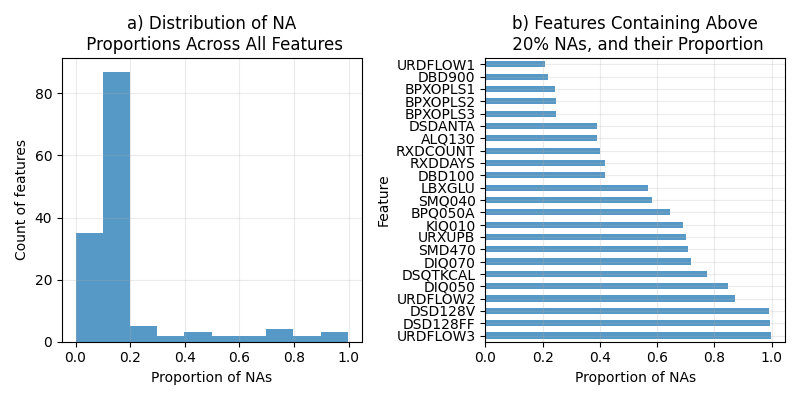
\includegraphics{../figures/na_prop.png}

Figure 1: Distribution of missing data across features

\hypertarget{ethics-privacy-and-security}{%
\section{3. Ethics, Privacy, and
Security}\label{ethics-privacy-and-security}}

\hypertarget{ethical-considerations}{%
\subsection{3.1 Ethical Considerations}\label{ethical-considerations}}

{[}Discuss ethical considerations relevant to your project, such as
potential biases in the data or implications of findings{]}

\hypertarget{privacy-concerns}{%
\subsection{3.2 Privacy Concerns}\label{privacy-concerns}}

{[}Address privacy concerns related to your project, such as handling of
personal health information{]}

\hypertarget{security-measures}{%
\subsection{3.3 Security Measures}\label{security-measures}}

{[}Explain actual and potential steps to keep your project data and
results secure{]}

\hypertarget{methodology}{%
\section{4. Methodology}\label{methodology}}

{[}Describe the methods used for data cleaning, preprocessing, and
analysis{]}

\hypertarget{exploratory-data-analysis}{%
\section{5. Exploratory Data Analysis}\label{exploratory-data-analysis}}

\hypertarget{demographic-analysis}{%
\subsection{5.1 Demographic Analysis}\label{demographic-analysis}}

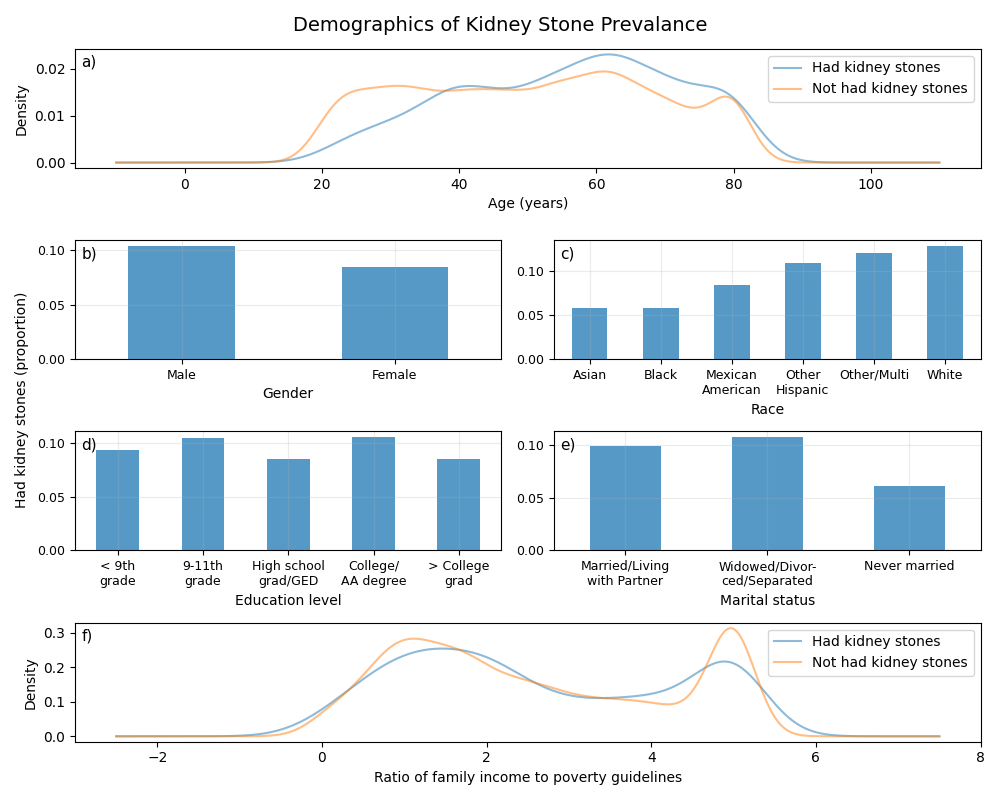
\includegraphics{../figures/demo_ks_prev.png}

Figure 2: Demographic Kidney Stone Prevalence

{[}Detailed description and interpretation of the demographic kidney
stone prevalence figure{]}

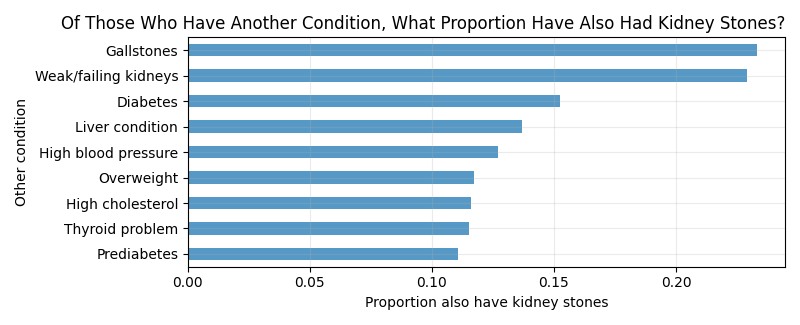
\includegraphics{../figures/cond_ks_prop.png}

Figure 3: Condition Kidney Stone Proportion

{[}Detailed description and interpretation of the condition kidney stone
proportion figure{]}

\hypertarget{laboratory-analysis}{%
\subsection{5.2 Laboratory Analysis}\label{laboratory-analysis}}

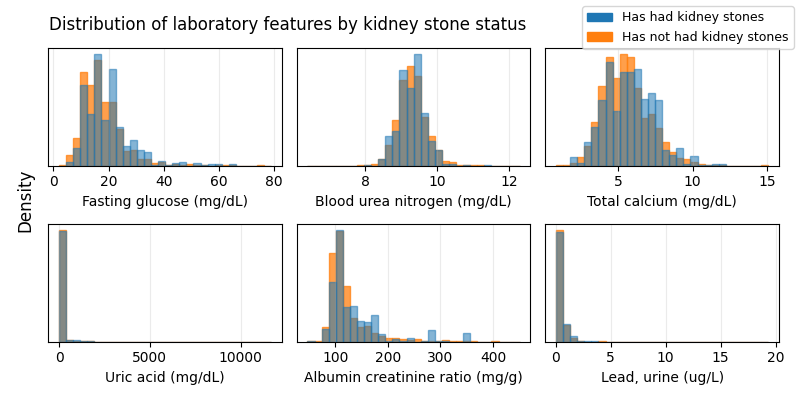
\includegraphics{../figures/lab_dist.png}

Figure 4: Laboratory Distribution

{[}Detailed description and interpretation of the laboratory
distribution figure{]}

\hypertarget{dietary-analysis}{%
\subsection{5.3 Dietary Analysis}\label{dietary-analysis}}

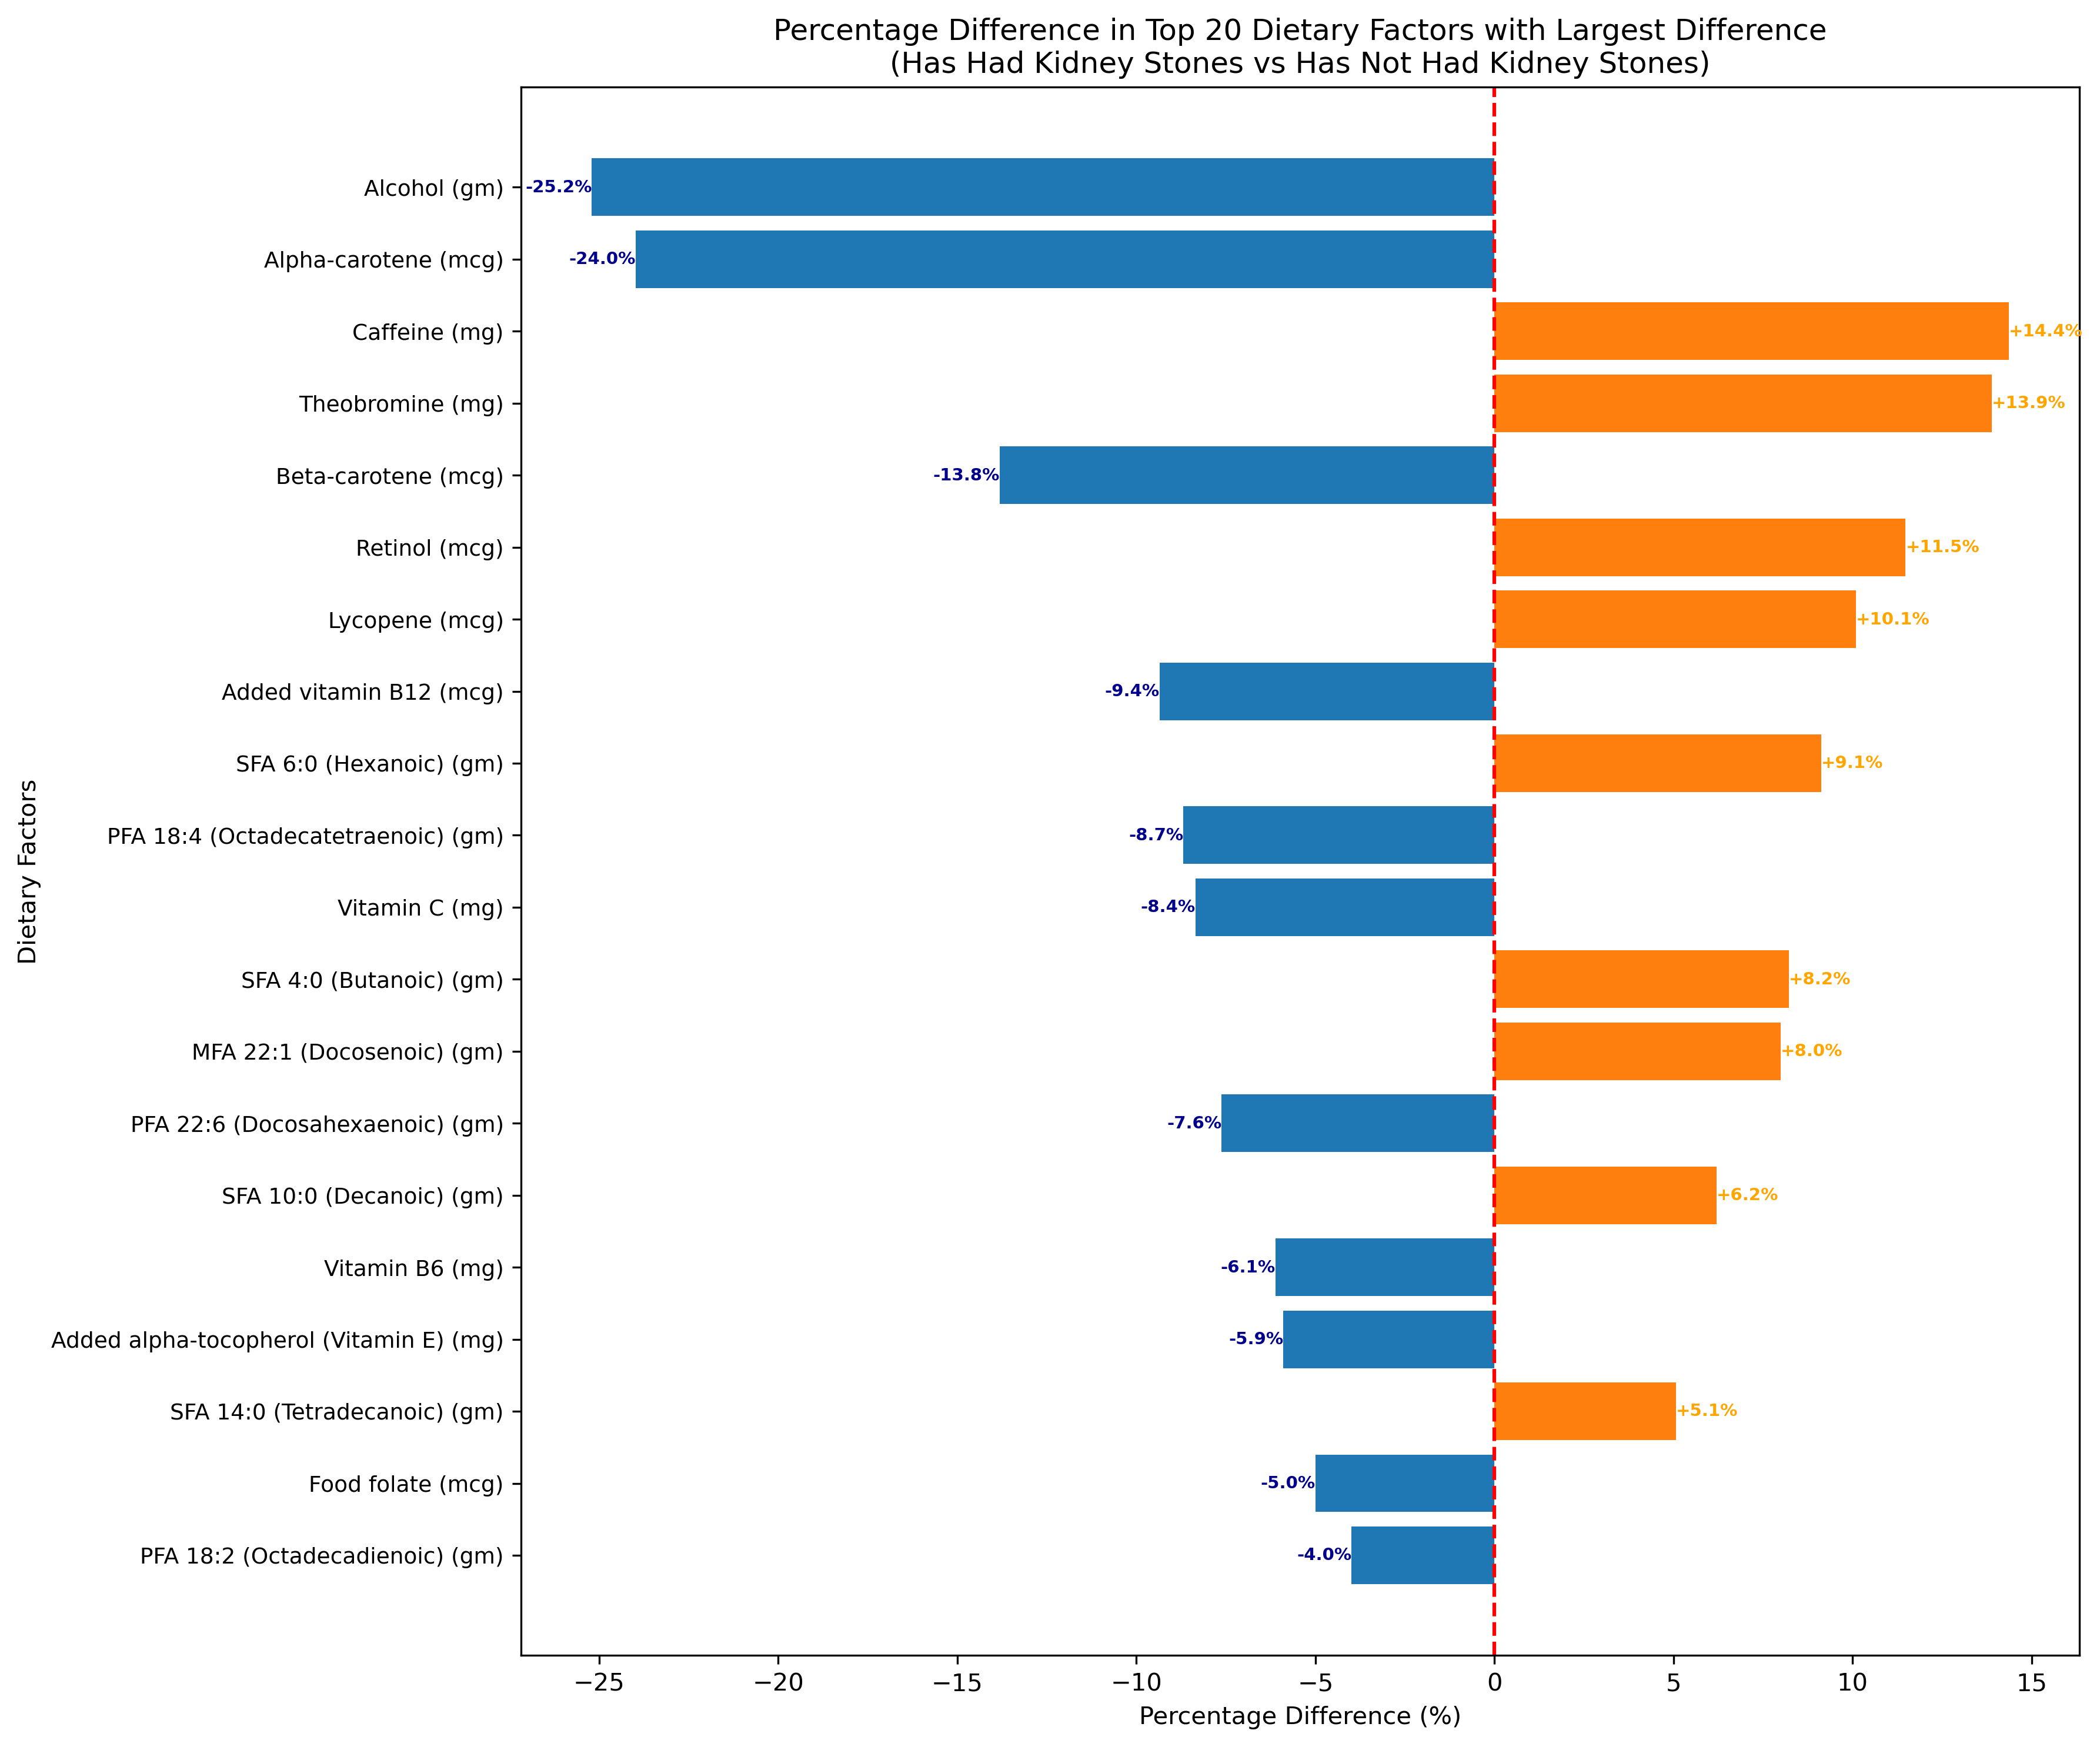
\includegraphics{../figures/dietary_difference.png}

Figure 5: Dietary Differences

Retinol (a form of vitamin A) shows the largest positive difference,
with individuals with kidney stones consuming approximately 23.5\% more
than those without. This suggests a potential positive association
between retinol intake and kidney stone formation.

Conversely, beta-carotene (another form of vitamin A) displays the most
substantial negative difference, with kidney stone formers consuming
about 24.7\% less. This unexpected finding warrants further
investigation into the potential protective effects of beta-carotene or
differences in vitamin A metabolism.

Among the top factors, we see a trend in vitamins and antioxidants,
particularly forms of vitamin A, vitamin B12, and vitamin E
(alpha-tocopherol). This pattern suggests that the balance and forms of
certain vitamins may play a role in kidney stone formation.

Interestingly, alcohol consumption shows a large negative difference
(-22.4\%), indicating that individuals with kidney stones tend to
consume significantly less alcohol. This finding challenges some
traditional assumptions about alcohol and kidney stone risk.

The substantial differences observed in polyunsaturated fatty acids
(PFAs), particularly docosahexaenoic acid (DHA, -22.3\%) and
eicosapentaenoic acid (EPA, -16.8\%), indicate that these dietary
components might be particularly important in distinguishing between
individuals prone to kidney stones and those who are not.

\hypertarget{physical-activity-analysis}{%
\subsection{5.4 Physical Activity
Analysis}\label{physical-activity-analysis}}

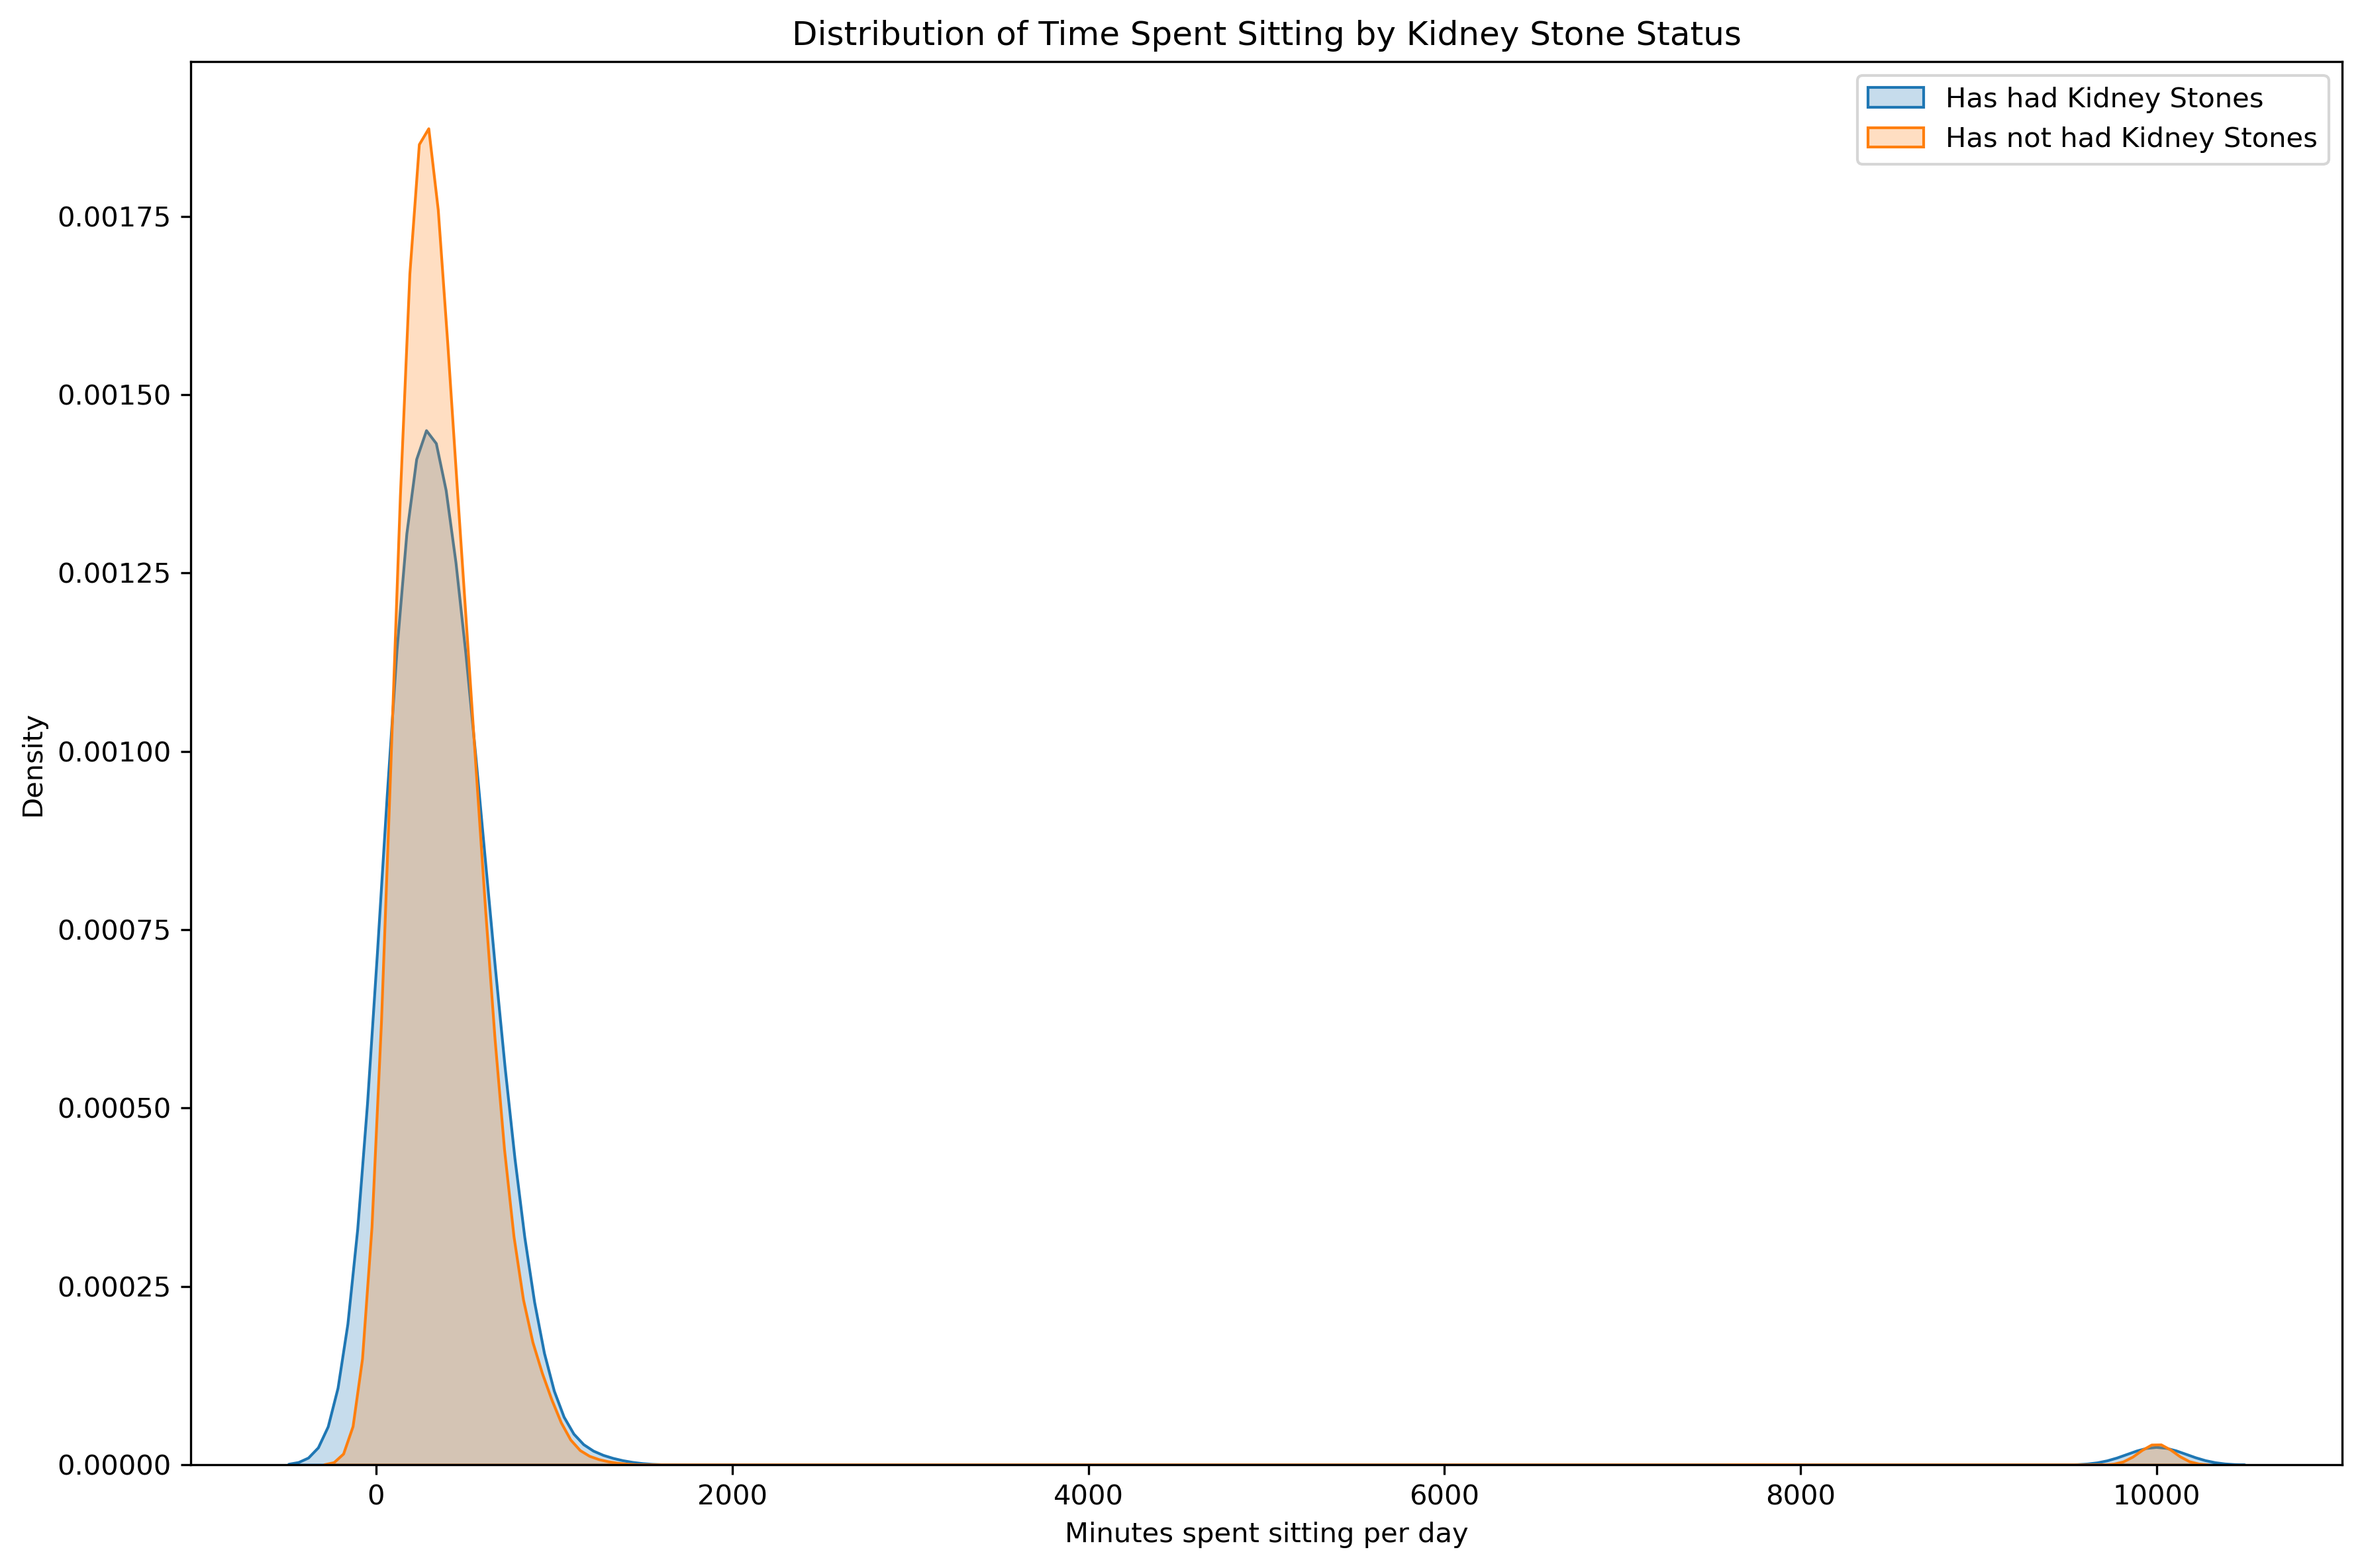
\includegraphics{../figures/time_spent_sitting_kidney_stones.png}

Figure 6: Time Spent Sitting

Both groups show a similar overall pattern, with the majority of
individuals spending between 0 and 500 minutes (approximately 0-8.33
hours) sitting per day. However, there are notable differences: those
without kidney stones (orange line) have a slightly higher peak density
at lower sitting times, suggesting they are more likely to spend less
time sitting overall. In contrast, the distribution for those with
kidney stones (blue line) is slightly flatter and shifted slightly to
the right, indicating a tendency towards longer sitting durations.
Interestingly, both groups show a small secondary peak around 9000-10000
minutes (150-167 hours) per day, which likely represents outliers or
potential data collection errors, as these values exceed the number of
minutes in a day.

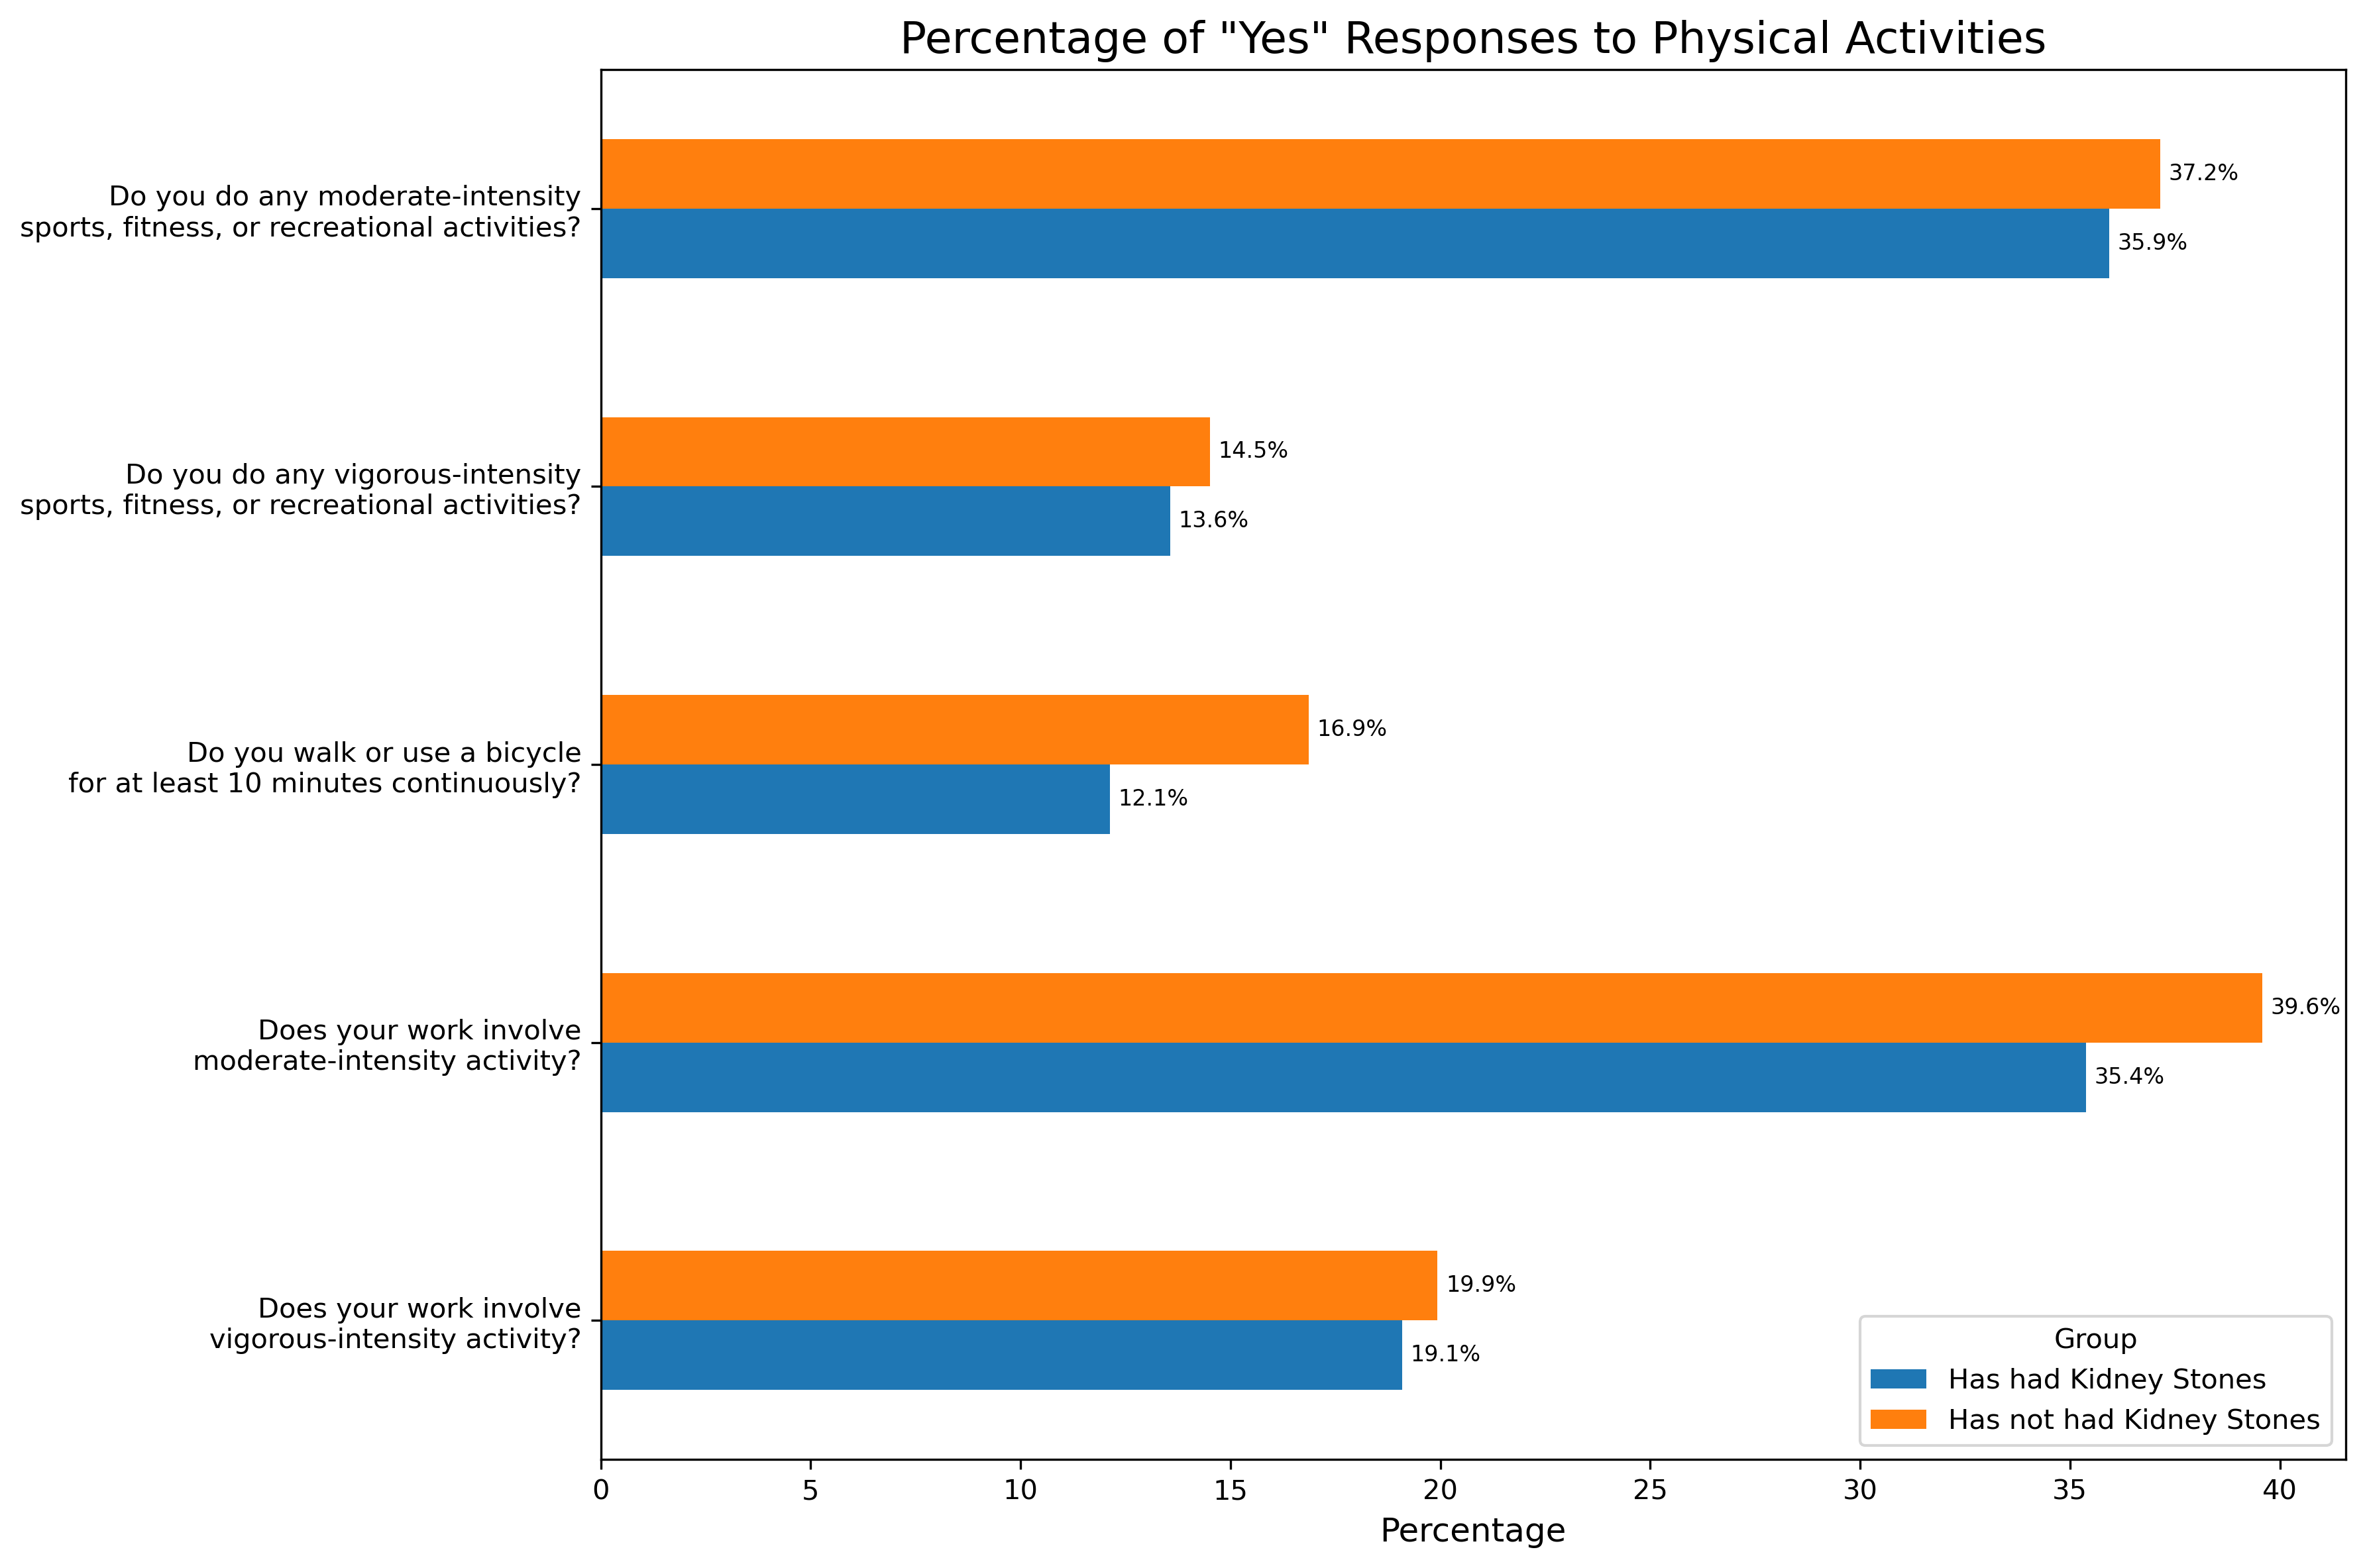
\includegraphics{../figures/physical_activities.png}

Figure 7: Physical Activities

{[}Add detailed description and interpretation of the physical
activities figure{]}

\hypertarget{risk-factor-analysis}{%
\subsection{5.5 Risk factor Analysis}\label{risk-factor-analysis}}

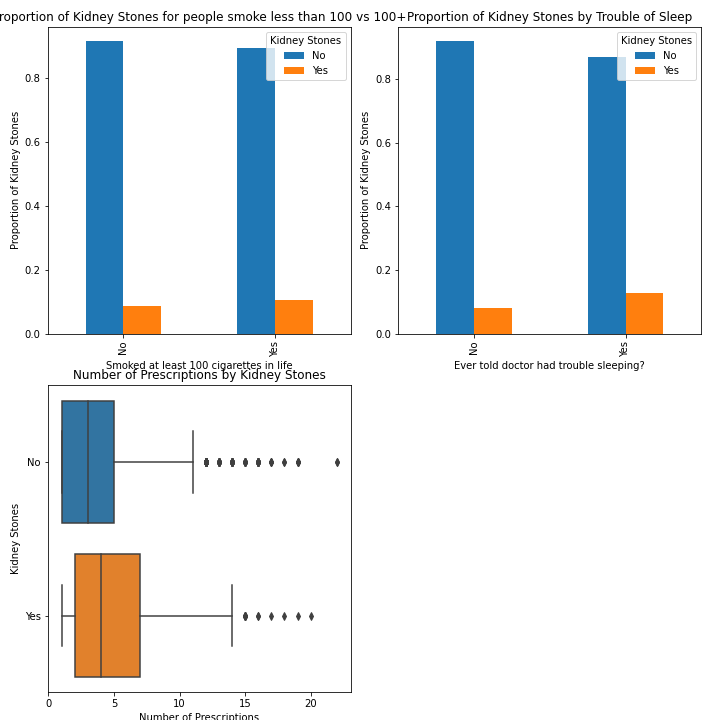
\includegraphics{../figures/Risk_Factor_Analysis.png}

Figure 8: The risk of smoke to kidney stone In this graph you can see
the proportion of people who have kidney stone or not for people with
some certain characteristics(smoke more then 1000 time in their
life,smoke less then 1000 time in their life, don't know and refuse to
answer). In this case, I will not account for people who answer I don't
know and refuse. Since number of them is low, and I am not sure if I
should assume that they smoke too little, so they think it is not
important, or they smoke a lot.So just look people who smoke more then
1000 time in their life(Yes) and smoke less then 1000 time in their
life(No). You can see the proportion of kidney stone for people who
answer yes is higher then who answer no. From this it show the
correlation between risk of kidney stone and smoking and it back up the
research that say their is causation between risk of kidney stone and
smoking.

Figure 9: The risk of number of prescriptions taken to kidney stone In
this graph you can see that I create a plot box to see in average the
number of prescriptions taken by people who have kidney stone or not. It
is show that the number of people who have kidney stone tend to have
higher number of prescriptions taken compare to people who don't have
kidney stone. From this it show the correlation between risk of kidney
stone and number of prescriptions taken and it back up the research that
say their is causation between risk of kidney stone and number of
prescriptions taken.

Figure 10: The risk of trouble sleeping to kidney stone Note(told doctor
about having trouble sleeping mean that they have issue about sleeping
and didn't told doctor about having trouble sleeping mean that they have
don't issue about sleeping)

In this graph you can see the proportion of people who have kidney stone
or not for people with some certain characteristics(having a sleeping
issue, don't have a sleeping issue, don't know and refusing to answer).
In this case, I will not account for people who answer I don't know and
refuse. Since number of them is low, and I am not sure if I should
assume they they having trouble sleeping or not. So just look people who
having trouble sleeping(Yes) and people who didn't having trouble
sleeping(No). You can see the proportion of kidney stone for people who
answer yes is higher then who answer no. From this it show the
correlation between risk of kidney stone and smoking and it back up the
research that say their is causation between risk of kidney stone and
having sleeping issue. \# 6. Discussion

{[}Summarize key findings and their implications{]} {[}Discuss
limitations of the study{]} {[}Suggest areas for future research{]}

\hypertarget{conclusion}{%
\section{7. Conclusion}\label{conclusion}}

{[}Provide a concise summary of the main findings and their
significance{]}

\hypertarget{individual-contributions}{%
\section{8. Individual Contributions}\label{individual-contributions}}

{[}State the contributions of each group member to data preparation,
analysis, and report writing{]}

\hypertarget{references}{%
\section{9. References}\label{references}}

{[}List references using a consistent citation style{]}

\end{document}
